The Compact Muon Solenoid (CMS) detector operates at the LHC at CERN. It was designed to operate in proton-proton (and lead-lead)
collisions at a center-of-mass energy of 14\TeV (5.5\TeV) and at
luminosities up to 10$^{34}$cm$^{-2}$s$^{-1}$
(10$^{27}$cm$^{-2}$s$^{-1}$). The CMS has cilindrical geometry and
its dimensions are a length of 21.5 m, a diameter of 14.6, and a total
weight of 12,500 tons. At the heart of the CMS detector system
lies a 4\unit{T} magnetic field produced by a large-bore superconducting
solenoid which encloses a silicon -- pixel and strips -- tracker, a homogeneous
lead-tungstate crystal electromagnetic calorimeter, and a brass-scintillator
sampling hadron calorimeter. Outside the superconducting solenoid lies
an iron yoke for magnetic flux-return instrumented with four stations
for muon detection. Forward sampling calorimeters extend the rapidity
coverage up to $\eta < 5$ and thus ensure good
hemiticity. Figure~\ref{fig:cmsDetector} shows an schematic representation
of the CMS detector and Figure~\ref{fig:cmsSlice} shows a cartoon
with a cross-sectional-slice view of the CMS detector along with
different particle detections.
\begin{figure}
 \centering
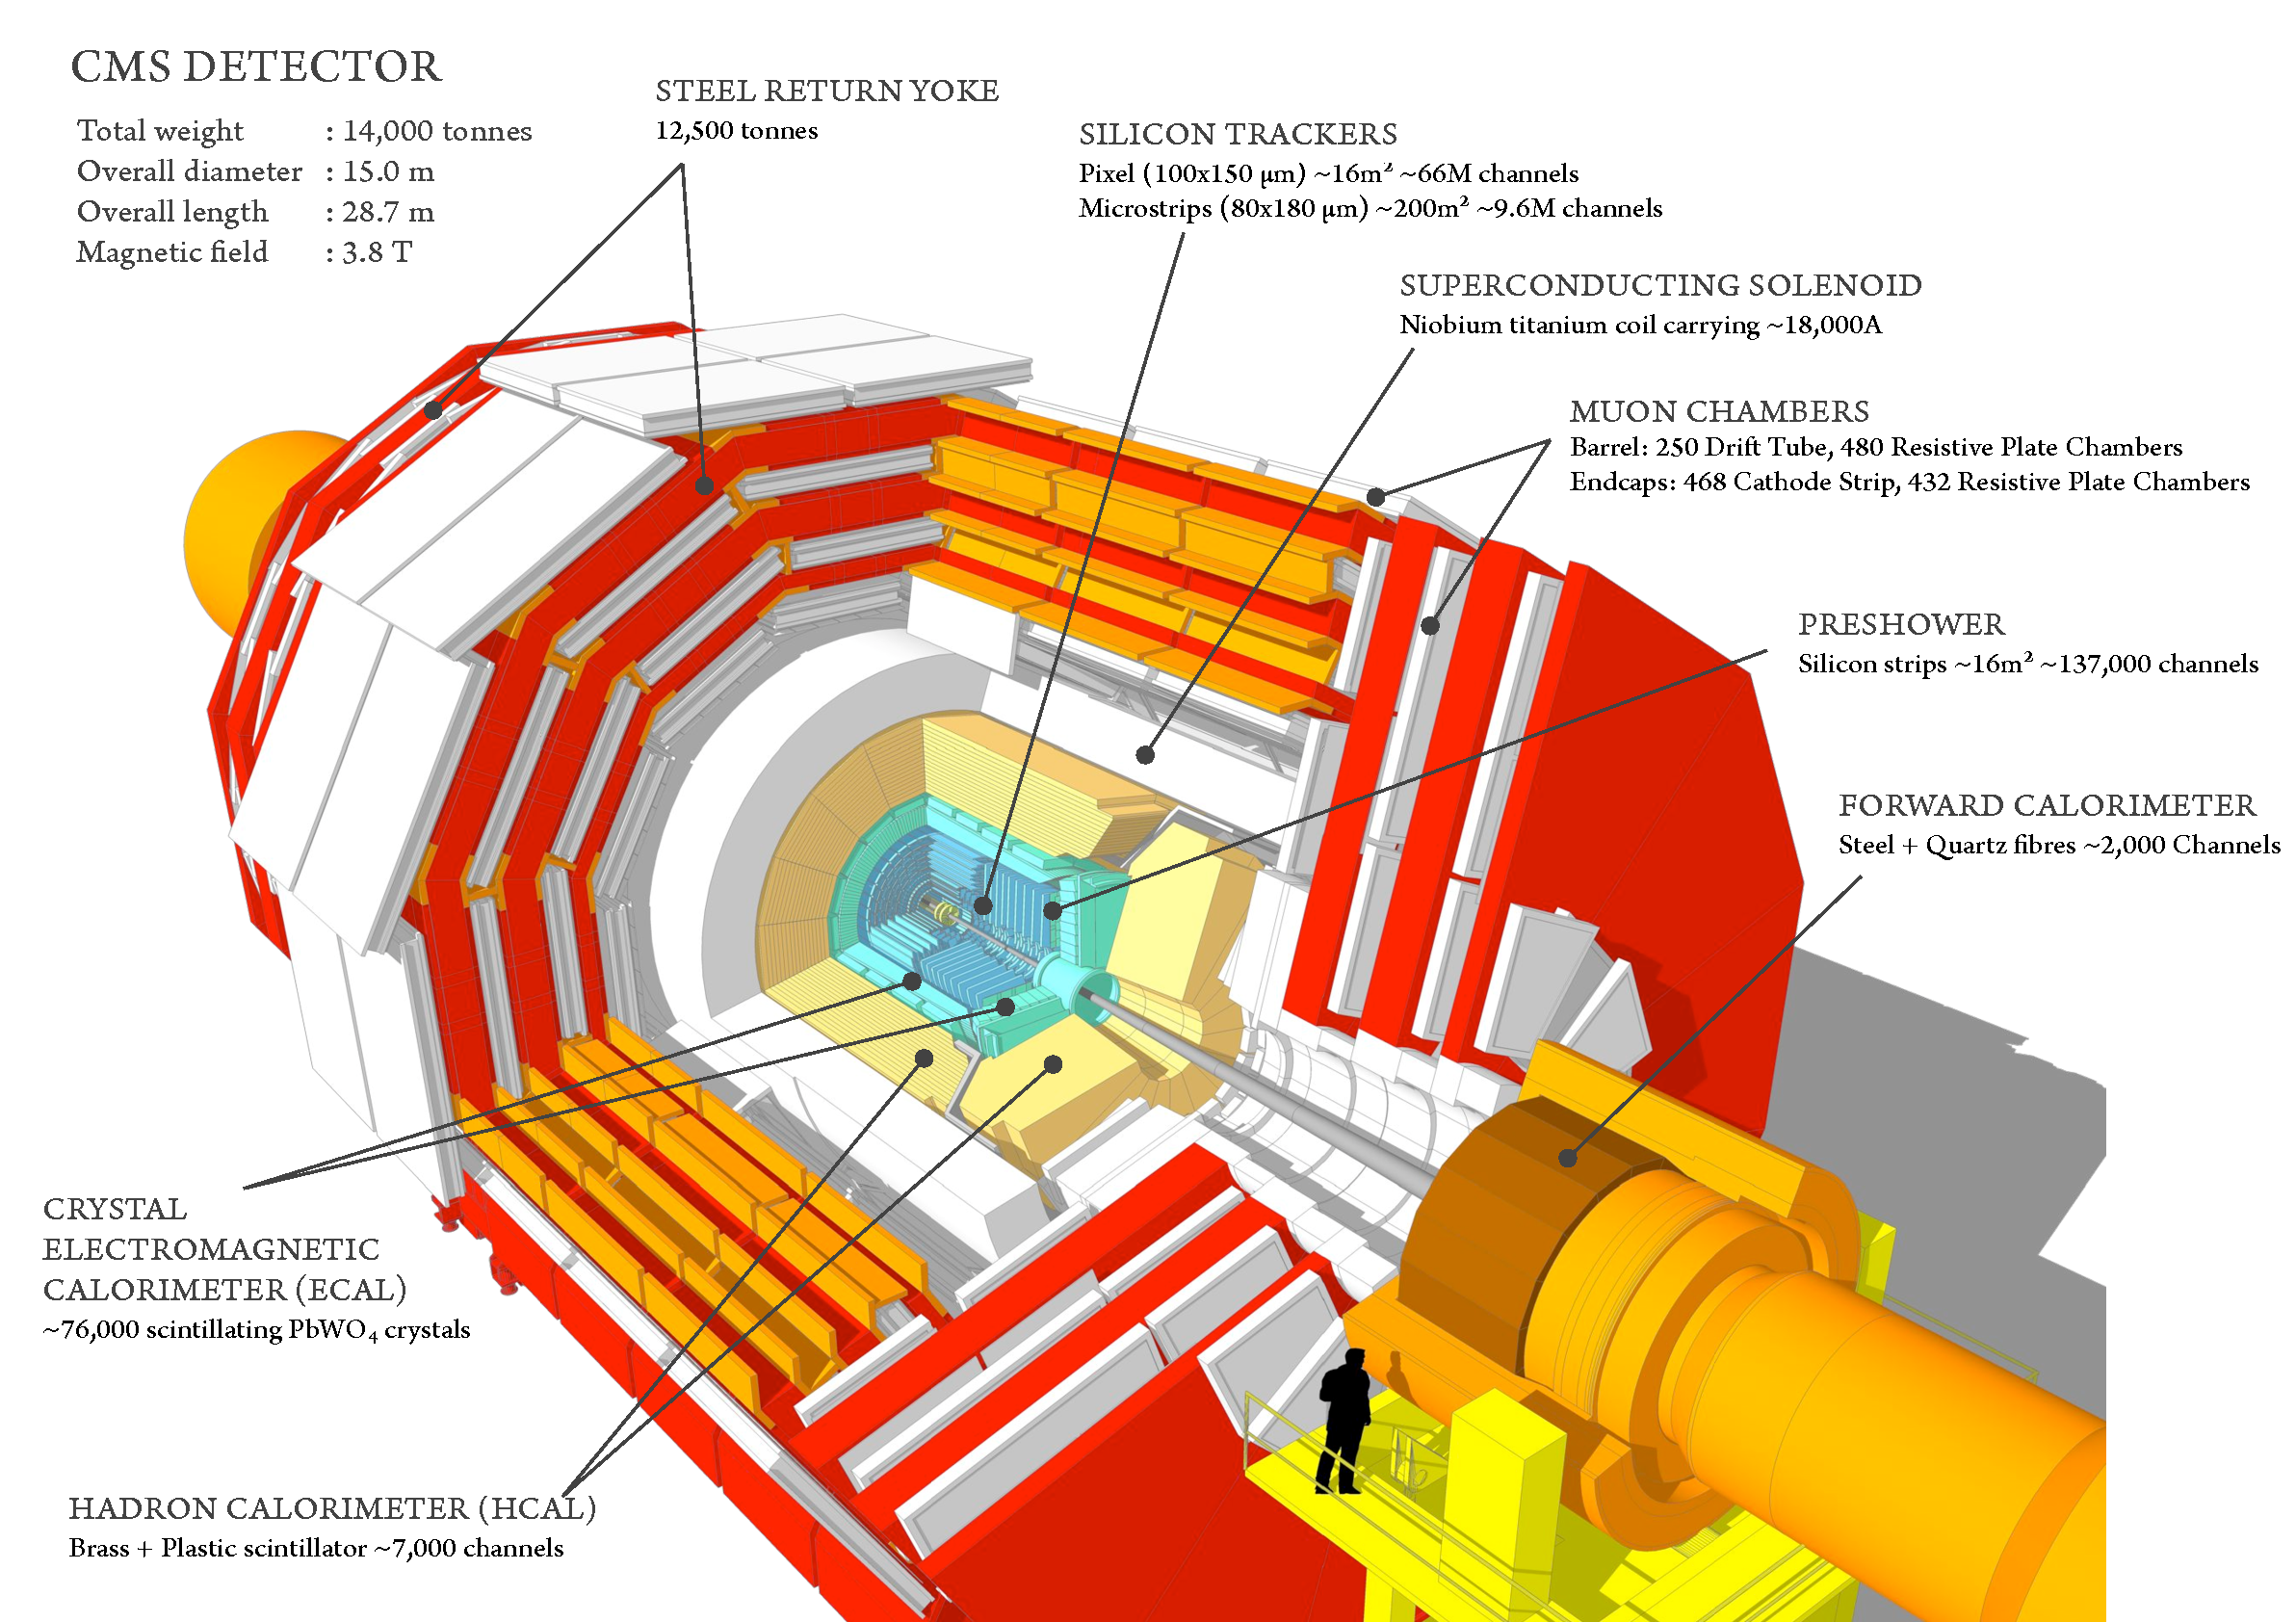
\includegraphics[width=0.99\textwidth]{CMS_DetectorFigures/cms_detector.png}
 \caption{A perspective view of the CMS detector.\label{fig:cmsDetector}}
\end{figure}
\begin{figure}
 \centering
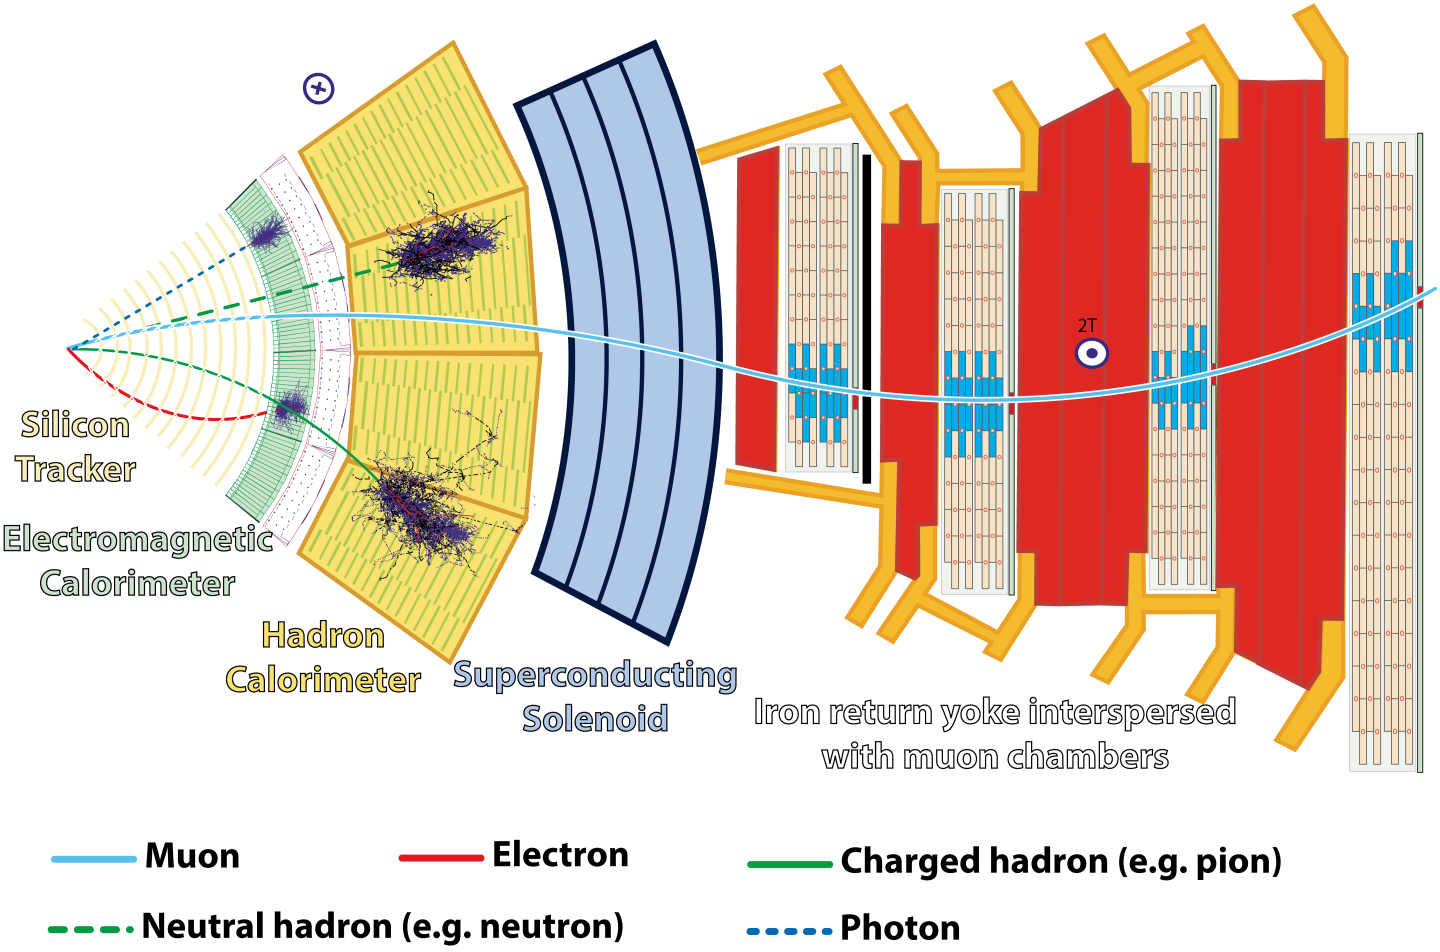
\includegraphics[width=0.99\textwidth]{CMS_DetectorFigures/CMSslice.png}
 \caption{A cross-sectional-slice view of the CMS detector. The
   different components of the detector are clearly labeled and
   different particle detections are depicted.\label{fig:cmsSlice}}
\end{figure}

This chapter presents an introduction to the CMS detector systems and
reconstruction algorithms. It is by no means a complete picture of the
CMS detector and its mostly based on Ref.~\cite{Chatrchyan:2008zzk}.
\section{The Tracker System}
The tracker is the innermost system of the CMS detector.
It was designed to measure efficiently and precisely the trajectories
of charged particles coming from the interaction points, as well as to
provide a precise reconstruction of the secondary vertices at each
bunch crossing. When running at the LHC designed conditions, every
buch crossing, i.e 25 ns, the number of proton-proton collision will
be about 20 and they will produce an average number of particles of about
1000. These conditions and the above requirements implied a highly granular and fast
response design. That being said, this design due to its high power
consumption requires an efficient cooling system which in turn is in
conflict with the goal of minimizing the material budget and thus
reduce unwanted interactions. In addition, the harsh radiation
environment that will deteriorate the detector performance posed
further challenges in its construction. Therefore, the system --
silicon sensors, readout, mechanical structures, granularity, etc --
was designed to operate for 10 year and satisfying the considerations
listed above. The CMS tracker is composed of three layers of pixels
detectors up to a radius of 10.2 cm, a 10-layer silicon strip tracker
up to a radious of 1.1 m, two endcap disks at each side of the barrel pixel detectors, 3
endcap disks at each side of the inner region of the strips (up to a
radius of 55 cm), and finally 9 disks covering the $|z|$ > 120 cm
regions starting a radious of 55 cm. More details about the tracker
layout will be given below and are summarized in
Figure~\ref{fig:trackerlayout}. The tracker covers up to
pseudorapidities of $|eta| < 2.5$ with a about 200 m$^2$ of active
silicon area implemented. 
\begin{figure}
 \centering
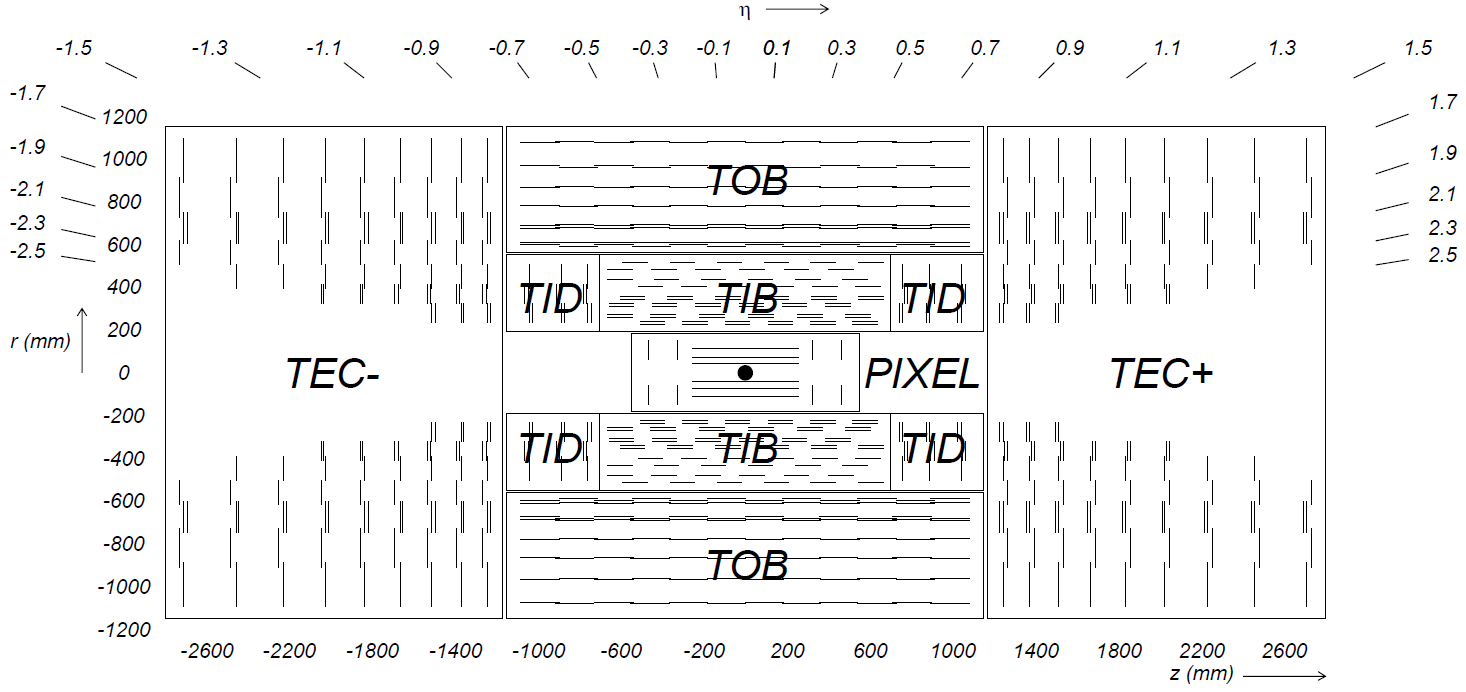
\includegraphics[width=0.99\textwidth]{CMS_DetectorFigures/TrackerLayout.png}
 \caption{A cross-sectional view of the silicon tracker layout. The
   different subsytems are clearly labeled.\label{fig:trackerlayout}}
\end{figure}

The inner pixel detector is composed of three 53-cm-long cylindrical layers at a
radii of 4.4, 7.3, and 10.2 cm. It is finallized by two disks of pixel
modules at each side extending from approximately 6 to 15 cm in radius.

\section{The Electromagnetic Calorimeter}
\section{The Hadronic Calorimeter}
\section{The Superconducting Solenoid}
\section{The Muon Chambers}